\section{141 --- Linked List Cycle}
Given a linked list $L$, determine if it has a cycle in it.
\par
To represent a cycle in the given linked list, we use an integer $P$ which represents the position (0-indexed) in the linked list where tail connects to. If $P$ is $-1$, then there is no cycle in the linked list.
\paragraph{Example 1:}
\begin{flushleft}
\textbf{Input}:$P = 1$, $L$ is shown as below
\begin{figure}[H]
\begin{tikzpicture}
[mynode/.style={draw,circle,minimum size=8mm, fill=gray!20!}]
\node(){};
\node[mynode](3) {3};
\node[mynode](2)[right=15mm of 3] {2};
\node[mynode](0)[right=15mm of 2] {0};
\node[mynode](M4)[right=15mm of 0] {-4};
\draw[>=stealth,->] (3) -- (2);
\draw[>=stealth,->] (2) -- (0);
\draw[>=stealth,->] (0) -- (M4);
\draw[>=stealth,->] (M4) to[bend left=45] (2);
\end{tikzpicture}
\end{figure}
\textbf{Output}: \texttt{true}
\\
\textbf{Explanation}: There is a cycle in the linked list, where tail connects to the second node.
\end{flushleft}
\paragraph{Example 2:}
\begin{flushleft}
\textbf{Input}: $P=0$, $L$ is shown as below
\begin{figure}[H]
\begin{tikzpicture}
[mynode/.style={draw,circle,minimum size=8mm, fill=gray!20!}]
\node(){};
\node[mynode](1) {1};
\node[mynode](2)[right=15mm of 1] {2};
\draw[>=stealth,->] (1) -- (2);
\draw[>=stealth,->] (2) to[bend left=45] (1);
\end{tikzpicture}
\end{figure}
\textbf{Output}: \texttt{true}
\\
\textbf{Explanation}: There is a cycle in the linked list, where tail connects to the first node.
\end{flushleft}
\paragraph{Example 3:}
\begin{flushleft}
\textbf{Input}: $P=-1$, $L$ is
\begin{figure}[H]
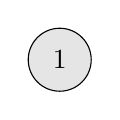
\begin{tikzpicture}
[mynode/.style={draw,circle,minimum size=8mm, fill=gray!20!}]
\node(){};
\node[mynode](1) {1};
\end{tikzpicture}
\end{figure}
\textbf{Output}: \texttt{false}
\\
\textbf{Explanation}: There is no cycle in the linked list.
\end{flushleft}
\paragraph{Follow up:}
\begin{itemize}
\item Can you solve it using $O(1)$ (i.e. constant) memory?
\end{itemize}
\subsection{Two Pointers}
Considering two pointers at different speed - a slow pointer and a fast pointer. The slow pointer moves one step at a time while the fast pointer moves two steps at a time.
\par
If there is no cycle in the list, the fast pointer will eventually reach the end and we can return \texttt{false} in this case.
\par
Now consider a cyclic list and imagine the slow and fast pointers are two runners racing around a circle track. The fast runner will eventually meet the slow runner. Why? Consider this case --- The fast runner is just one step behind the slow runner. In the next iteration, they both increment one and two steps respectively and meet each other.
\par
How about other cases? For example, we have not considered cases where the fast runner is two or three steps behind the slow runner yet. This is simple, because in the next or next's next iteration, this case will be reduced to case mentioned above.
\setcounter{algorithm}{0}
\begin{algorithm}[H]
\caption{Two Pointers}
\begin{algorithmic}[1]
\Procedure{HasCycle}{$H$}
\If{$H=\texttt{null}$}
\State \Return \texttt{false} \Comment Empty list
\EndIf
\State $F:=H$ \Comment The fast pointer
\State $S:=H$ \Comment The slow pointer
\While{$F\neq \texttt{null}$ \textbf{and} $F.\texttt{next}\neq \texttt{null}$}
\State $F\gets F.\texttt{next}$
\State $F\gets F.\texttt{next}$ \Comment $F$ move forward two steps
\State $S\gets S.\texttt{next}$ \Comment $S$ move forward one step
\If{$F=S$}
\State \Return \texttt{true}
\EndIf
\EndWhile
\State \Return \texttt{false}
\EndProcedure
\end{algorithmic}
\end{algorithm}